\documentclass[titlepage = firstcover]{scrartcl}
\usepackage[aux]{rerunfilecheck}
\usepackage{fontspec}
\usepackage[main=ngerman, english, french]{babel}

% mehr Pakete hier
\usepackage{expl3}
\usepackage{xparse}

%Mathematik------------------------------------------------------
\usepackage{nicefrac}
\usepackage{amsmath}   % unverzichtbare Mathe-Befehle
\usepackage{amssymb}   % viele Mathe-Symbole
\usepackage{mathtools} % Erweiterungen für amsmath
\usepackage{dsfont}
\usepackage[
  math-style=ISO,    % \
  bold-style=ISO,    % |
  sans-style=italic, % | ISO-Standard folgen
  nabla=upright,     % |
  partial=upright,   % /
]{unicode-math}% "Does exactly what it says on the tin."
\usepackage[section, below]{placeins}

% Laden von OTF-Mathefonts
% Ermöglich Unicode Eingabe von Zeichen: α statt \alpha

\setmathfont{Latin Modern Math}
%\setmathfont{Tex Gyre Pagella Math} % alternativ zu Latin Modern Math
\setmathfont{XITS Math}[range={scr, bfscr}]
\setmathfont{XITS Math}[range={cal, bfcal}, StylisticSet=1]

\AtBeginDocument{ % wird bei \begin{document}
  % werden sonst wieder von unicode-math überschrieben
  \RenewDocumentCommand \Re {} {\operatorname{Re}}
  \RenewDocumentCommand \Im {} {\operatorname{Im}}
}
\usepackage{mleftright}
\setlength{\delimitershortfall}{-1sp}
\usepackage[version=4]{mhchem}

%Sprache----------------------------------------------------------
\usepackage{microtype}
\usepackage{xfrac}
\usepackage[autostyle]{csquotes}    % babel
\usepackage[german, unicode, pdfusetitle]{hyperref}
\usepackage{bookmark}
\usepackage[shortcuts]{extdash}
%Einstellungen hier, z.B. Fonts
\usepackage{booktabs} % Tabellen

\setlength{\parindent}{0pt}

\title{V601 - Der Franck-Hertz Versuch}
\author{
  David Gutnikov\\
  \href{mailto:david.gutnikov@udo.edu}{david.gutnikov@udo.edu}\\
  Lasse Sternemann\\
  \href{mailto:lasse.sternemann@udo.edu}{lasse.sternemann@udo.edu}
}
\date{Bearbeitet am 7.07.2020}

\begin{document}
    \maketitle
    \newpage
    \tableofcontents
    \newpage

    \section{Zielsetzung}
        Mithilfe dieses Versuches lässt sich die Ionisationsenergie/die Energiedifferenz zwischen dem 1. angeregten Zustand und dem Grundzustand von Quecksilber bestimmen.

    \section{Theorie}
        \subsection{Einleitung}
            Mit dem Franck-Hertz-Versuch ist es möglich Anregungsenergien von Atomen eines Gases zu messen und somit Aussagen über die Struktur dieser Atome zu treffen.
            Die Verfahren, um diesen Zweck zu erfüllen werden unter dem Begriff der Atomspektroskopie zusammengefasst.
            Es gibt zwei solche Methoden, die benutzt werden.

            Bei der Ersten wird ein Stoff elektromagnetischer Strahlung aus gesetzt und die Absorption und Emission werden beobachtet. Unter Einfluss von elektrischen und magnetischen Feldern spalten sich die Energieniveaus der Elektronenhülle in eine feinere Struktur auf und es ist möglich weitere Daten aufzunehmen.

            Die zweite Methode, zu der der Franck-Hertz-Versuch zählt, sind die Elektronenstoßexperimente. Hierbei werden Elektronen mit einer bekannten Energie auf die Atome geschossen und der Energieverlust der Elektronen wird gemessen.

        \subsection{Allgemeiner Aufbau des Franck-Hertz-Versuches}
            \begin{figure}[h]
                \centering
                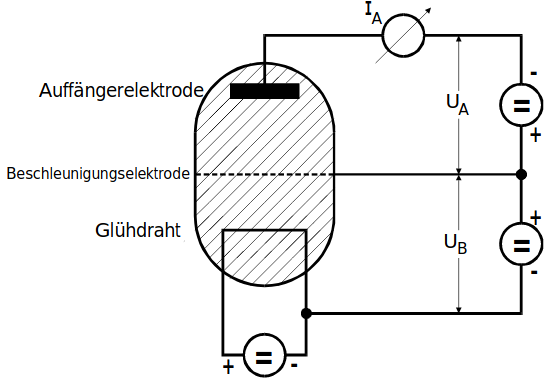
\includegraphics[width = 0.6\textwidth]{Bilder/Aufbau_FranckHertz.png}
                \caption{Der schematische Aufbau der Franck-Hertz-Versuches. [1]}
                \label{fig:Aufbau_FranckHertz}
            \end{figure}

            \FloatBarrier

            In einem evakuirten Glasgefäß befindet sich ein Quecksilbertropfen.
            Dieser verdampft abhängig von der Temperatur $T$ verschieden stark und das Gefäß füllt sich mit Hg-Gas.
            Die Dampfdichte des Gases hängt nur von der Temperatur ab und lässt sich durch diese relativ leicht kontrollieren.

            Auf einer Seite des Gefäßes befindet sich ein Glühdraht/-kathode, welcher durch einen Gleichstrom erhitzt wird.
            Dabei treten aufgrund des glühelektrischen Effektes Elektronen aus dem Draht aus.

            In der Mitte des Glases ist eine netzförmige Elektrode plaziert.
            An den Glühdraht und die Beschleunigungselektrode wird eine Spannung $U_{\text{B}}$ angelegt, sodass die austretenden Elektronen in Richtung der netzförmigen Elektrode beschleunigt werden.

            Auf der gegenüberliegenden Seite zum Draht befindet sich eine massive Auffängerelektrode, an der der Auffängerstrom abfließt.
            Auch wird eine Spannung $U_{\text{A}}$ an die Beschleunigungselektrode und und die Auffängerelektrode gelegt.
            Dadurch werden die Elektronen abgebremst die Anzahl der an der Auffängerelektrode ankommenden Elektronen wird reguliert.

        \subsection{Funktionsweise}
            Nach Durchlaufen der Beschleunigungsspannung erhalten die Elektronen eine kinetische Energie von
            \begin{equation*}
                \frac{1}{2} m v^2_{\text{vor}} = e_0 U_{\text{B}}
            \end{equation*}
            mit der Elektronenmasse $m$, der Elementarladung $e_0$ und der Endgeschwindigkeit $v_{\text{vor}}$.
            Dabei wird angenommen, dass die Anfangsgechwindigkeit der Elektronen 0 ist.

            Damit die Elektronen die Auffängerelektrode erreichen können muss für die z-Komponente ihrer Geschwindigkeit $v_{\text{z}}$ gelten:
            \begin{equation*}
                \frac{1}{2} m v^2_{\text{z}} \geq e_0 U_{\text{A}}
            \end{equation*}
            Ist $v_{\text{z}}$ zu klein, schaffen es die Elektronen nicht die Gegenspannung zu überwinden, fallen zur netzförmigen Elektrode zurück und fließen als Strom an ihr ab. \\

            Während des Fluges können die im Gefäß verteilten Hg-Atom auf zwei Arten mit den Elektronen interagieren.

            Erstens, trifft ein Elektron auf ein Atom, passiert ein elastischer Stoß. Dabei ist der Energieverlust des Elektrons vernachlässigbar klein, da die Stoßpartner ein Massenverhältnis von $\nicefrac{m}{M} \approx \nicefrac{1}{2000}$ zueinander haben. Beim zentralen Stoß würde z.B. die Energieabgabe betragen:
            \begin{equation*}
                \Delta E = \frac{4 m M}{(m + M)^2} E \approx 1,1 \cdot 10^{-5} E
            \end{equation*}
            Jedoch können die Elektronen leicht an den vergleichsweise schweren Atomen gestreut werden.
            Diese elastischen Stöße treten im Bereich der niedrigen Elektronenenergien am häufigsten auf und bewirken also keine Änderung des Betrages der kinetischen Energie, sondern eine Änderung der Richtung der Geschwindigkeit und damit eine Änderung der z-Komponente der Energie. \\

            Zweitens, nimmt die kinetische Energie der Elektronen mit steigender Beschleunigungsspannung zu, sodass die Energie gleich der Differenz zwischen dem 1. angeregten Zustand und dem Grundzustand des Hg-Atoms $E_1 - E_0$ ist.
            Dann ist es nämlich in der Lage des Hg-Atom anzuregen, d.h. die Energie $E_1 - E_0$ wird auf das Atom übertragen und ein Elektron von einem tieferen Energieniveau springt in ein höheres Energieniveau.

            Nach einer Relaxationszeit von ca. $10^ {-8}$s geht das Atom unter Emission eines Lichtquants der Energie
            \begin{equation*}
                h \nu = E_1 - E_0
            \end{equation*}
            wieder in den Grundzustand über.\\

            Um die Energiedifferenz zwischen den Energieniveaus zu bestimmen, wird die Beschleunigungsspannung $U_{\text{B}}$ bei einer konstanten Gegenspannung $U_{\text{A}}$ erhöht.

            Ist $U_{\text{B}}$ größer als $U_{\text{A}}$ geworden, steigt der Auffängerstrom stark an, da jetzt fast allen Elektronen durch die Beschleunigungsspannung genug Energie mitgegeben wurde, um die Gegenspannung überwinden zu können.

            Doch die Elektronenenergie $e_0 U_{\text{B}}$ steigt weiter und kurz vor der netzförmigen Elektrode wird der Wert
            \begin{equation}
                e_0 U_{\text{B}} = E_1 - E_0
                \label{eqn:spannung}
            \end{equation}
            erreicht.
            Jetzt fällt der Strom wieder abrupt auf null herab, weil die Elektronen beim Anregen der Atome ihr Energie verlieren und nicht genug Zeit haben, um eine genügend hohe Geschwindigkeit aufzubauen, um die Gegenspannung zu überwinden.

            Steigt $U_{\text{B}}$ noch weiter, wandert der Bereich der Anregung der Atome immer näher in Richtung des Drahtes, da die Elektronen immer schneller die Energie erreichen, um ein Atom anregen zu können.

            Mir wachsendem $U_{\text{B}}$ steigt der Strom wieder schnell und fällt wieder auf null herab, weil die Elektronen nach der 1. Anregung wieder genug Energie bekommen, dass sie die Atome ein zweites Mal anregen können.

            Und so geht es noch ein paar Mal weiter.

            Dieser ideale Kurvenverlauf ist in \autoref{fig:IdealerAuffaengerstrom} dargestellt. Der Abstand zwischen den Peaks bleibt gleich und ist anhand von \autoref{eqn:spannung}:
            \begin{equation*}
                U_{1} = \frac{1}{e_0}(E_1 - E_0)
            \end{equation*}

            \begin{figure}[h]
                \centering
                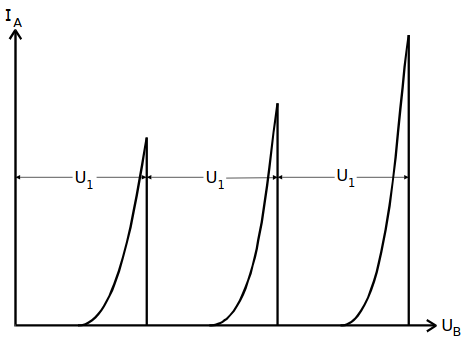
\includegraphics[width = 0.45\textwidth]{Bilder/IdealerAuffaengerstrom.png}
                \caption{Der ideale Verlauf einer Kurve, wo der Auffängerstrom $I_{\text{A}}$ gegen die Beschleunigungsspannung $U_{\text{B}}$ aufgetragen wird. [1]}
                \label{fig:IdealerAuffaengerstrom}
            \end{figure}

            \FloatBarrier

        \subsection{Die tatsächliche Franck-Hertz-Kurve}
            Die tatsächliche Franck-Hertz-Kurve unterscheidet sich etwas von der idealen Kurve. Sie ist nicht so spitz zulaufend und breiter. Das hängt von den folgenden drei Effekten.
            \subsubsection{Einfluss des Kontaktpotentials}
                Für die den Glühdraht und die Beschleunigungselektrode werden Materialien mit verschiedenen Austrittsarbeiten verwendet.
                Der Draht hat eine viel kleinere Austrittsarbeit $\Phi_{\text{G}}$ als die Beschleunigungselektrode $\Phi_{\text{B}}$. Dies führt dazu, dass auch bei niedrigen Temperaturen eine hohe Emissionsrate gegeben ist. 
                
                \begin{figure}[h]
                    \centering
                    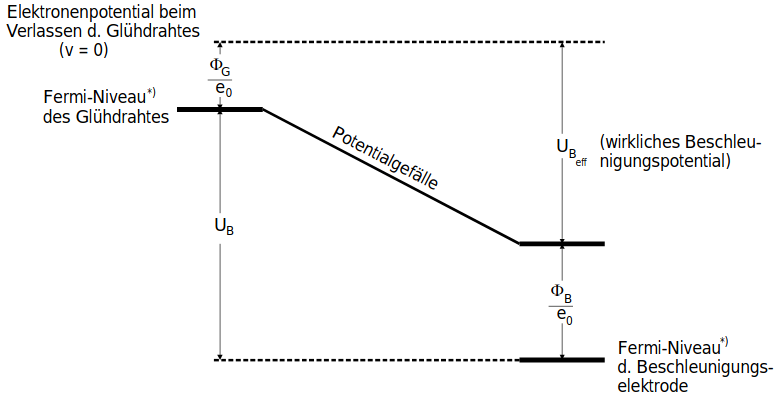
\includegraphics[width = 0.8\textwidth]{Bilder/Austrittsarbeit.png}
                    \caption{Hier ist die tatsächliche Potentialdifferenz zwischen Gühdraht und Beschleunigungselektrode dargestellt. [1]}
                    \label{fig:Austrittsarbeit}
                \end{figure}

                \FloatBarrier

                Aus \autoref{fig:Austrittsarbeit} ist ersichtlich, dass für die tatsächliche Beschleunigungsspannung $U_{\text{B,eff}}$ gilt:
                \begin{equation*}
                    U_{\text{B}} + \frac{\Phi_{\text{G}}}{e_0} = U_{\text{B,eff}} + \frac{\Phi_{\text{B}}}{e_0} \qquad \implies \qquad U_{\text{B,eff}} = U_{\text{B}} - \underbrace{\frac{1}{e_0}(\Phi_{\text{B}} - \Phi_{\text{G}})}_{K}
                \end{equation*}
                Die Franck-Hertz-Kurve ist also um dieses sogenannte Kontaktpotential $K$ nach rechts verschoben, da die angelegte Beschleunigungsspannung um $K$ höher eingestellt werden muss, damit die effektive Beschleunigungsspannung ausreicht um die Hg-Atome anzuregen.

            \subsubsection{Einfluss des Energie-Spektrums der Elektronen}
                Es wurde hier zuerst angenommen, dass die Elektronen keine Anfangsgeschwindigkeit kurz nach dem Austreten aus dem Glühdraht besitzen. Doch jedes Elektron bringt eine Energie mit, da das Energiespektrum der freien Elektronen in einem Metall durch die Fermi-Dirac-verteilung beschrieben wird.

                Also sind unter den Elektronen verschiedene Anfangsgeschwindigkeiten vertreten, die bei null anfangen und mit schnell abnehmender Häufigkeit kontinuirlich steigen. Aus dem selben Grund fangen die Elektronenenergien nach Durchlaufen der Beschleunigungsspannung bei $U_{\text{B,eff}}$ an und steigen kontinuirlich mit schnell abnehmender Häufigkeit. \\

                Deswegen wird die zur Anregung nötige Elektronenenergie nicht mehr von allen Elektronen gleichzeitig erreicht und die Franck-Hertz-Kurve wird breiter und fällt nicht mehr so abrupt auf null herab, sondern sie nähert sich einem Minimum. Anschaulich sind die Peaks nicht mehr so spitz.

            \subsubsection{Einfluss der elastischen Stöße}
                Passieren elastische Stöße von Elektronen mit Hg-Atomen auf dem Beschleunigungsweg zwischen dem Glühdraht und der Beschleunigungselektrode, haben sie keine große Auswirkung auf den Auffängerstrom, da sie wieder beschleunigt werden.

                Elastische Stöße zwischen der Beschleunigungselektrode und Auffängerelektrode tragen jedoch zu einer deutlichen Veränderung des Auffängerstromes bei. Durch die von den Stößen stammenden Richtungsänderungen werden die z-Komponenten der Elektrongeschwindigkeiten stark verändert und viele Elektronen schaffen es nicht mehr die Gegenspannung zu überwinden. \\

                Die Kurve wird breiter und flacher.

            \subsubsection{Einfluss des Dampfdruckes}
                Damit möglichst viele Stöße passieren können, muss die freie Weglänge $\overline{w}$ der Hg-Atome klein gegen den Abstand $a$ des Drahtes von der Beschleunigungselektrode sein.

                Die Weglänge kann durch den Sättigungsdruck $p_{\text{sät}}$ des Hg-Gases reguliert werden, welcher seinerseits nur durch die Umgebungstemperatur beeinflussbar ist:

                \begin{align}
                    &\overline{w} \; [\text{cm}] = \frac{0,0029}{p_{\text{sät}}} \; [p\text{ in mbar}] \\[10pt]
                    &p_{\text{sät}}(T) = 5,5 \cdot 10^7 \exp\Bigl(-\frac{6876}{T}\Bigr) \quad [p\text{ in mbar, } T\text{ in K}]
                \end{align}

                Es gibt einen idealen Arbeitsbereich für den Franck-Hertz-Versuch, mit einem $\overline{w}$ um einen Faktor 1000 bis 4000 kleiner als $a$.

                Ist der Dampfdruck zu groß, wird die freie Weglänge zu klein und es passieren viel mehr elastische Stöße, sodass durch die Richtungsänderungen der Auffängerstrom stark abnimmt.

                Ist der Dampfdruck zu gering, wird die freie Weglänge zu groß und die Elektronen fliegen durch das Gas ohne mit den Atomen zu interagieren. Dabei erreichen sie mit steigender Beschleunigungsspannung so große Energieen, dass es theoretisch möglich wäre die Atome auf höhere Energieniveaus anzuregen. Die Stoßwarscheinlichkeit ist jedoch zu klein, um diesen Effekt messen zu können.

                \begin{figure}[h]
                    \centering
                    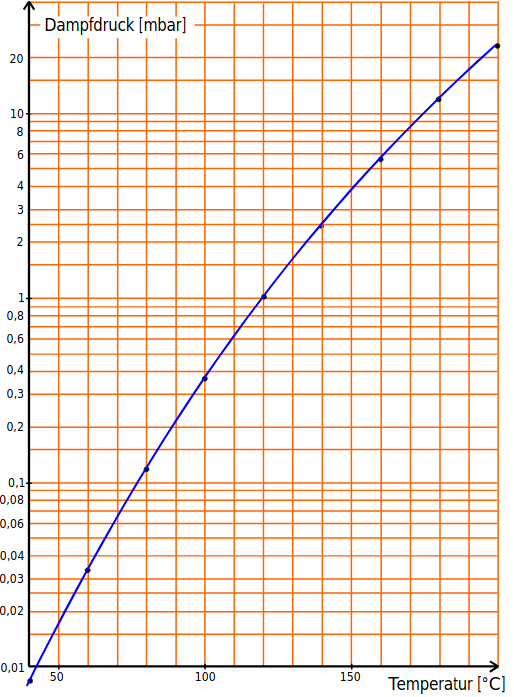
\includegraphics[width = 0.8\textwidth]{Bilder/Dampfdruckkurve.png}
                    \caption{Hier ist die Dampfdruckkurve des Hg-Gases dargestellt. Dabei ist der Sättigungsdampfdruck gegen die Umgebungstemperatur aufgetragen. [1]}
                    \label{fig:Dampfdruckkurve}
                \end{figure}

                \FloatBarrier
    
    \newpage
    \section{Aufbau}

        \begin{figure}[h]
            \centering
            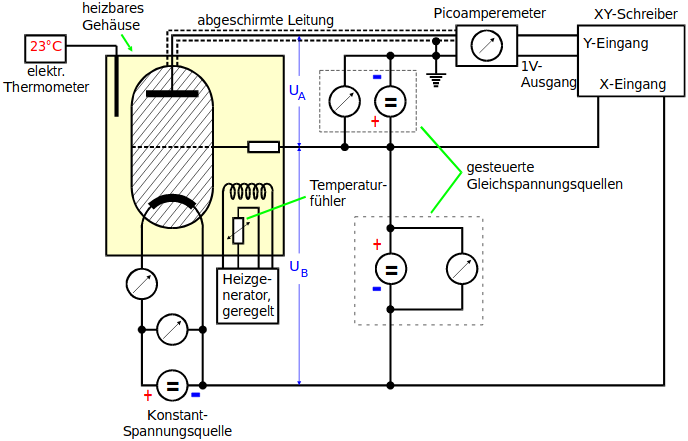
\includegraphics[width = 0.8\textwidth]{Bilder/Aufbau.png}
            \caption{Hier ist der konkret für den Versuch benutzte Aufbau abgebildet. [1]}
            \label{fig:Aufbau}
        \end{figure}

        \FloatBarrier

        Wie schon zuvor beim allgemeinen Aufbau erklärt, werden die Stromkreise der Heizspannung, Beschleunigungsspannung und Gegenspannung mit Gleichstrom betrieben.
        Der Aufbau besteht aus dem Glasgefäß mit dem Glühdraht, der netzförmigen Elektrode und der massiven Auffängerelektrode, den Apparaten zur Temperaturregelung und den dazugehörigen Messapparaten. \\

        Das Glasgefäß ist in einem heizbaren Gehäuse untergebracht, welches an einen Heizgenerator und an ein elektrisches Thermometer angeschlossen ist. \\

        Ein Picoamperemeter misst den Auffängerstrom und ist mit dem Y-Eingang eines XY-Schreiber verbunden, sodass die Kurven anhand der Messwerte für der Strom sofort gezeichnet werden können.

        Zum X-Eingang des Schreibers wird entweder die Beschleunigungsspannung oder die Gegenspannung verbunden.

        An den Spannungsquellen lässt sich einstellen, dass eine Spannug stetig steigen oder fallen soll.

    \newpage
    \section{Durchführung}
        Vor der Aufnahme einer Messreihe wird der Nullpunkt der beiden Skalen in der linken unteren Ecke festgelegt. 
        Zuerst wird ein unempfindlicher Bereich für die Skalen gewählt und dann solange runtergeregelt, bis eine gut erkennbare Kurve gezeichnet wird. \\

        Kurz vor einer Messung wird der Stift des Schreibers auf ein Blatt Millimeterpapier aufgesetzt und die Spannung auf der x-Achse wird auf steigend gestellt. \\

        Nach der Messung kann der Y-Eingang ausgestöpselt werden und die Spannung wird je einen oder zwei Volt fallen gelassen (je nachdem wie groß die Schrittweite der Skala sein soll), bevor sie gestoppt wird und durch ein Aufsetzen des Stiftes ein Punkt markiert wird. So kann ganz einfach eine Skala für die Spannung unter die Kurve gezeichnet werden.

        \subsection*{Aufgabe a)}
            Hier wird der Auffängerstrom in Abhängigkeit von der Gegenspannung $U_{\text{A}}$ bei einer festen Beschleunigungsspannung $U_{\text{B}} = 11$V gemessen. Die Spannung durchläuft dabei ein Intervall von 0V bis 47V.

            Zuerst wird eine Messreihe bei Zimmertemperatur $T = 27,7°$C aufgenommen. Danach wird der die Temperatur am Heizgenerator durch eine höhere Spannung auf $T = 151°$C hochgeregelt und es wird eine zweite Messreihe aufgenommen.
        
        \subsection*{Aufgabe b)}
            Hier wird genauso vorgegangen wie in Aufgabe a), nur dass der Auffängerstrom jetzt in Abhängigkeit von $U_{\text{B}}$ bei einem festen $U_{\text{A}} = 1$V gemessen. Die Spannung durchläuft dabei ein Intervall von 0V bis 47V.


            Die Messung wird bei einem $T = 197,1°$C durchgeführt.
    \newpage
    \section{Auswertung}    
        \subsection{Mittlere freie Weglänge}
            Zunächst wird überprüft, ob die freie Weglänge $\overline{w}$ die Bedingung erfüllt, um ca. das tausendfache kleiner als der Abstand a zwischen Glühkathode und Beschleunigungsanode zu sein.
            Die freien Weglängen berechnen sich über Formel xx und werden daraufhin zur Berechnung des Verhältnis zwischen a=1cm und $\overline{w}$ genutzt.

            \begin{table}[h]
                \centering
                \caption{In der Tabelle sind die den Temperaturen zugehörigen mittleren Weglängen der Gasatome, sowie das zugehörige Verhältnis zur Beschleunigungsdistanz a zu sehen.}
                \label{tab:TabGasdruck}

                \begin{tabular}{c  c c}
                    \toprule
                    {$T \; [\text{K}] $} & {$\overline{w} \; [\text{m}\cdot 10^{-6}]$} &  {$\frac{\text{a}}{\overline{w}}$} \\
                    \midrule
                    300,85 & 4500 & 2,3 \\
                    424,15 & 5,8 &  1800  \\
                    443,15 & 2,9 &  3500  \\
                    470,25 & 1,2 &  8500  \\
                    \bottomrule
                \end{tabular}

            \end{table}

        \newpage
        \subsection{Differentielle Energieverteilung}
            Zunächst wird berechnet wie viel Volt ein Kästchen auf dem Graphen der jeweiligen Temperatur des xy-Schreibers entspricht. Dazu wird folgende Formel benutzt, die zunächst aus den 
            einzelnen Abständen $d_i$ den durchschnittlichen Abstand zwischen den 1 Volt Markierungen bestimmt und daraus die Volt pro Kästchen.

            \begin{equation*}
                \text{Volt/Kästchen} \; \text{[V]} = \sum_{i=1}^{n} \frac{1}{d_i}
            \end{equation*}

            \FloatBarrier

                \begin{figure}[h]
                  \centering
                  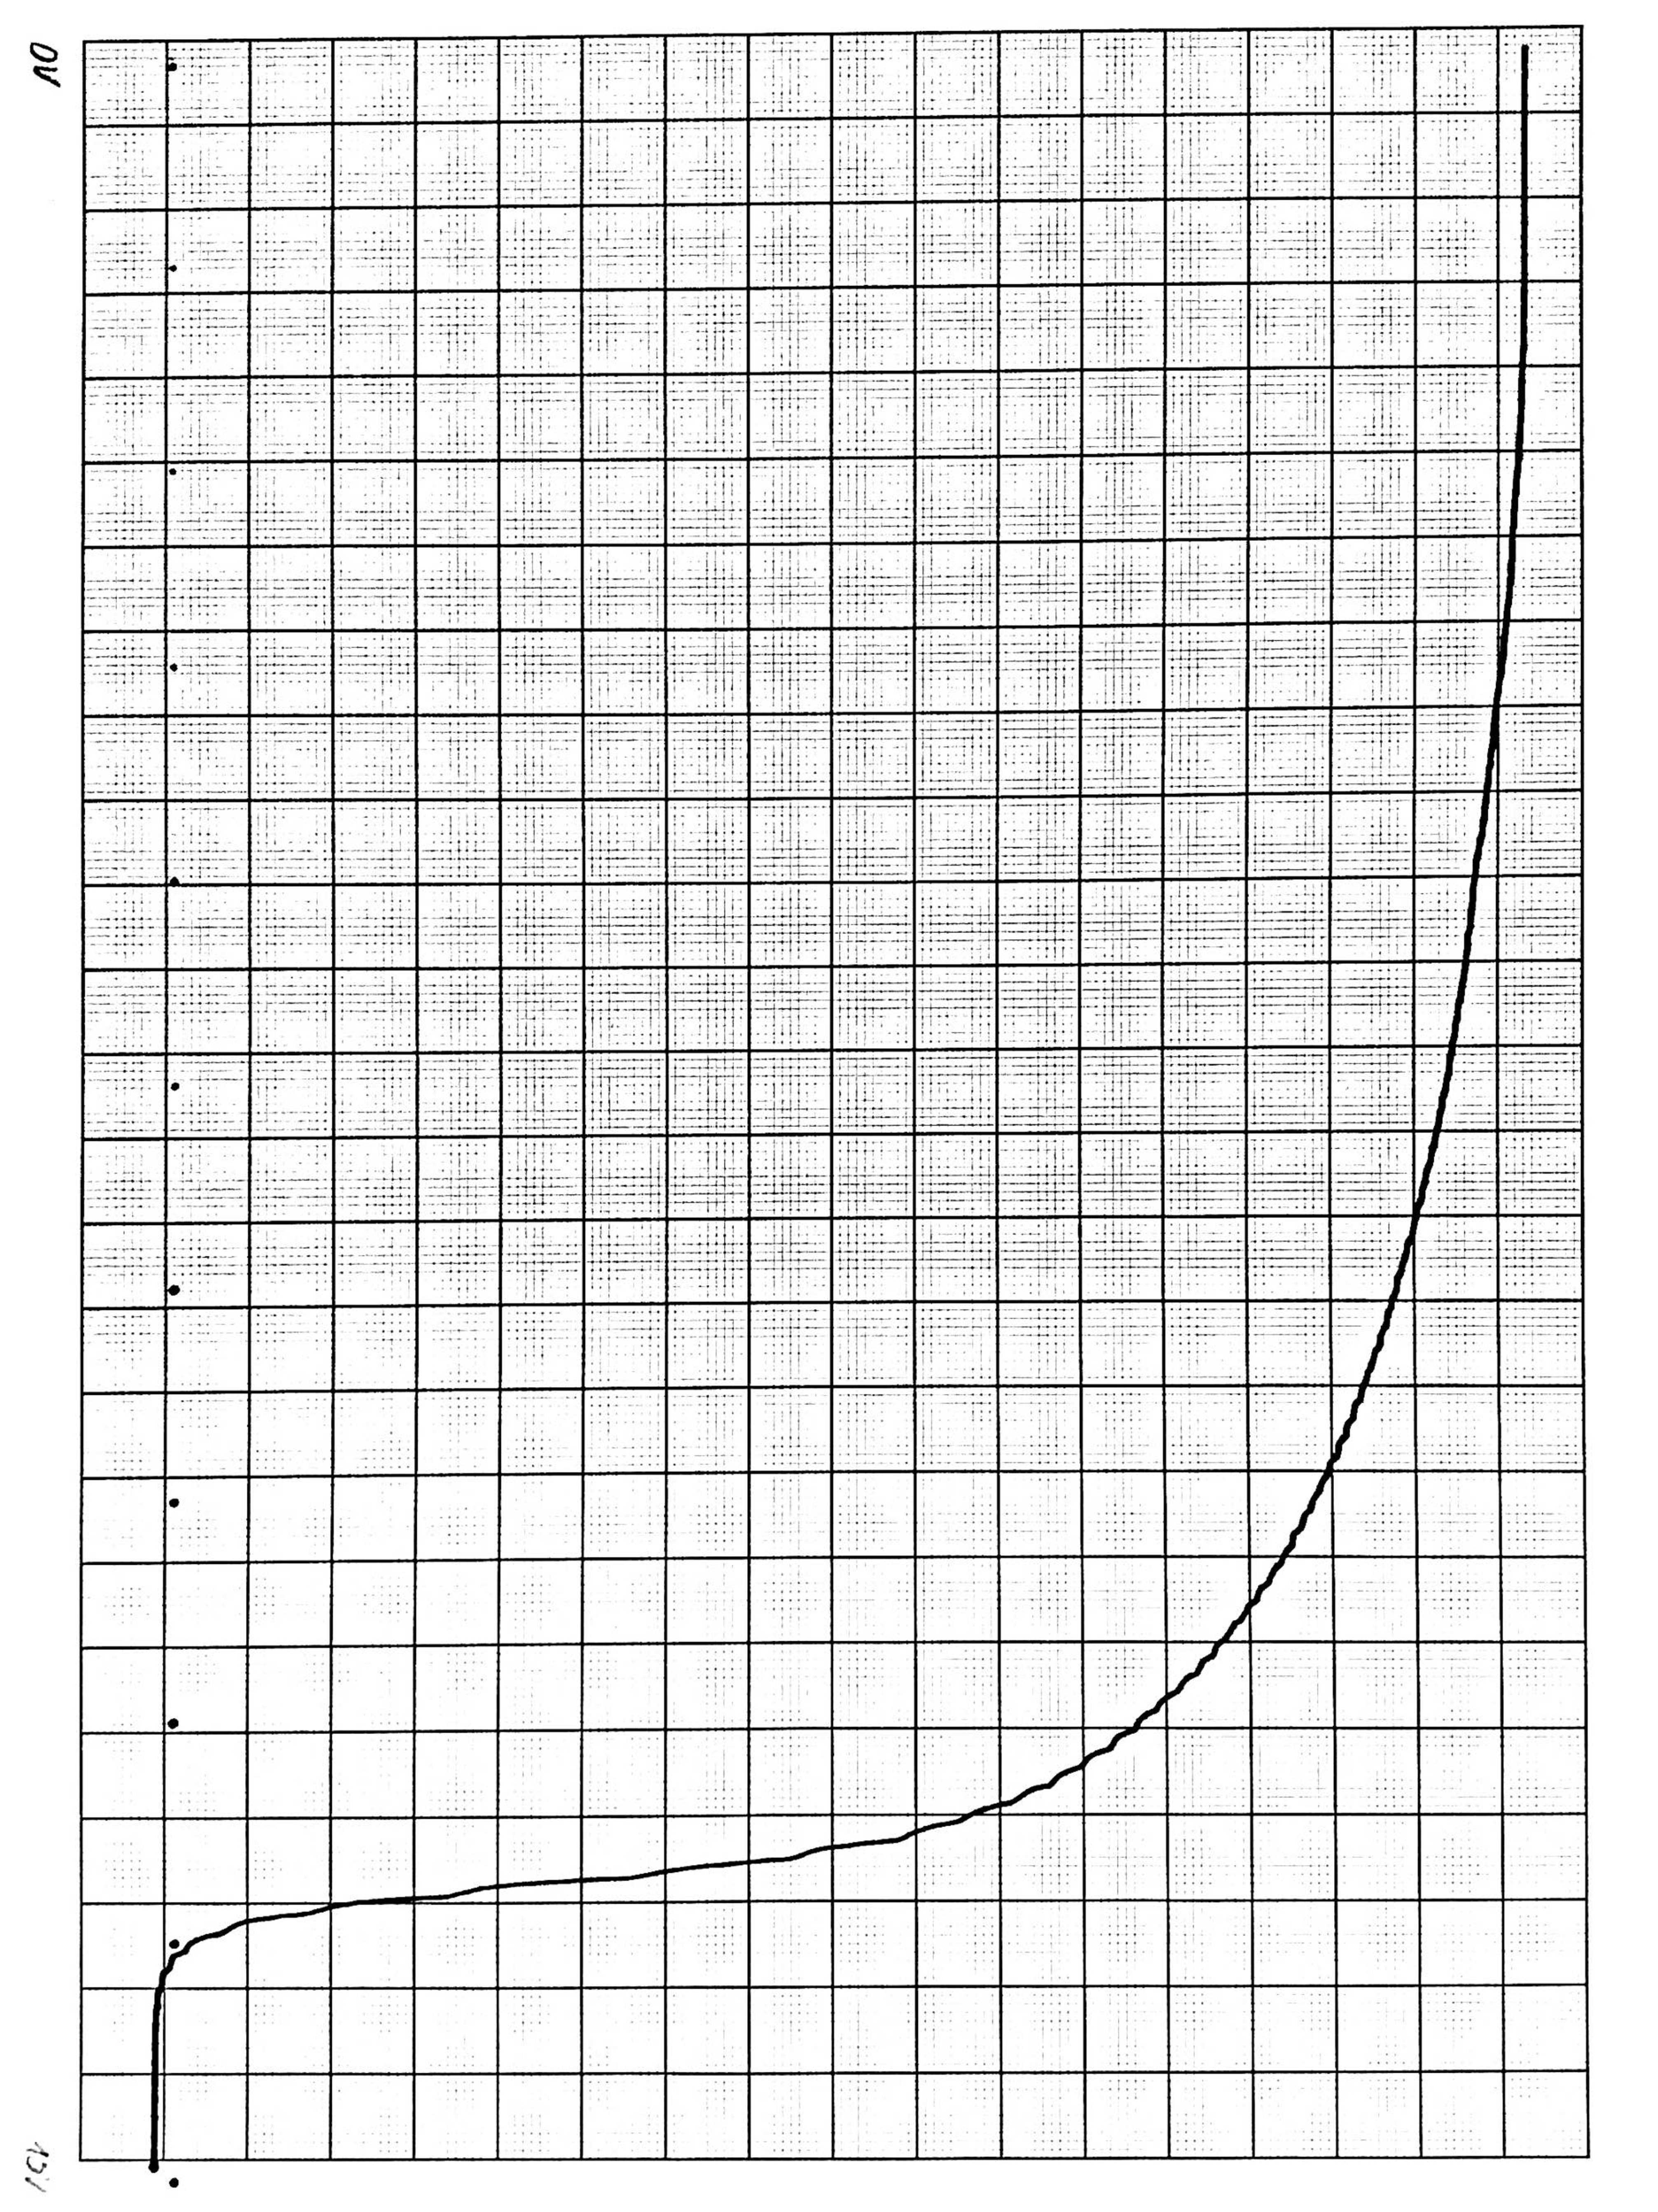
\includegraphics[width = 0.8\textwidth, angle=90]{T300.pdf}
                  \caption{In der Abbildung ist die integrale Energieverteilung der ausgelösten Elektronen bei einer Temperatur von 300,85 Kelvin zu sehen. Dazu wird der gemessene Kathodenstrom, der losgelösten Elektronen, in Abhängigkeit von der Bremsspannung aufgetragen. Der Abstand zwischen zwei schwarzen Punkten beträgt 1 Volt.}
                  \label{fig:Bild300}
                \end{figure}

                \begin{figure}[h]
                    \centering
                    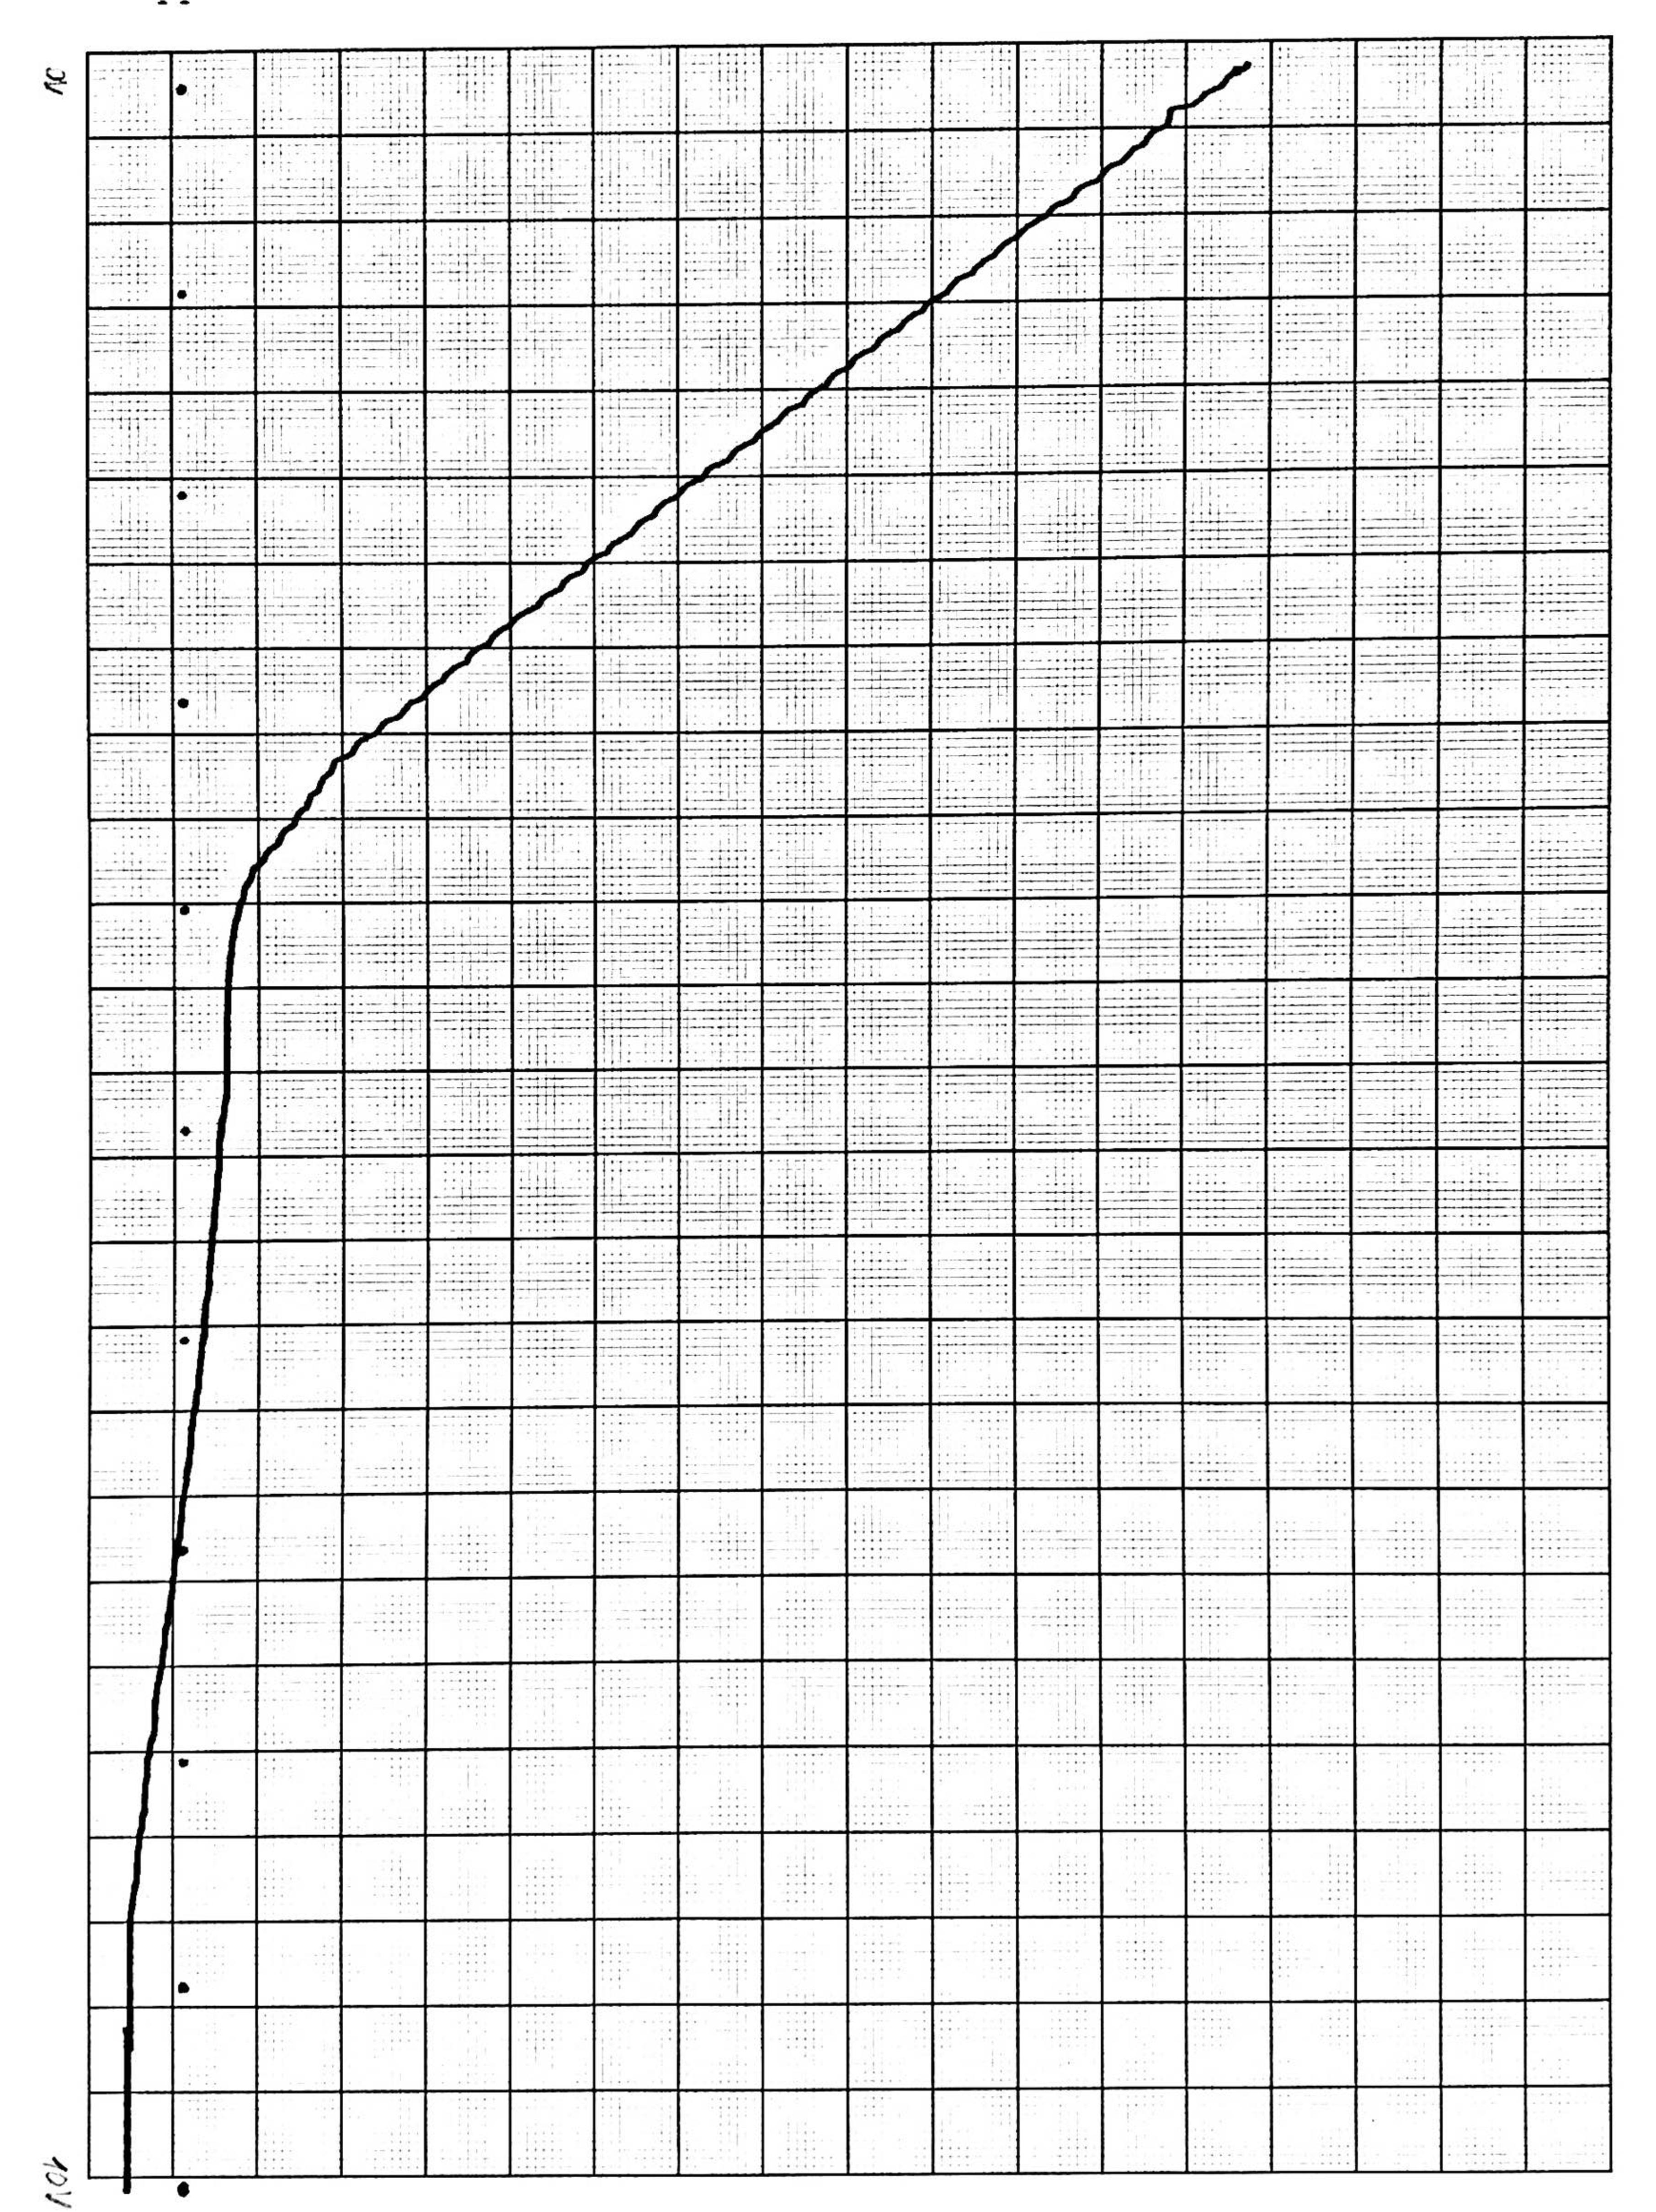
\includegraphics[width = 0.8\textwidth, angle=90]{T424.pdf}
                    \caption{In der Abbildung ist nun die integrale Energieverteilung der ausgelösten Elektronen bei einer Temperatur von 424,15 Kelvin zu sehen. Dazu wird der gemessene Kathodenstrom, der losgelösten Elektronen, erneut in Abhängigkeit von der Bremsspannung aufgetragen. Der Abstand zwischen zwei schwarzen Punkten beträgt wieder 1 Volt.}
                    \label{fig:Bild424}
                \end{figure}

            \FloatBarrier

            \noindent            

            \begin{table}[h]
                \centering
                \caption{In der Tabelle sind zunächst die Anzahlen der Kästchen zwischen den 1V-Markierungen zu sehen. Aus diesen wurde die durchschnittliche Skalierung der x-Achse in mV/Kästchen berechnet.}
                \label{tab:Tabelle1}

                \begin{tabular}{c c c c c}
                    \toprule
                    {} & {300,85 K} & {424,15 K} \\
                    \midrule
                    Kästchen/V    & 24 & 24 \\
                                  & 24 & 24 \\
                                  & 24 & 25 \\
                                  & 25 & 24 \\
                                  & 24 & 26 \\
                                  & 24 & 25 \\
                                  & 25 & 25 \\
                                  & 26 & 25 \\
                                  & 26 & 27 \\
                                  & 28 & 24 \\
                    \o \; mV/Kästchen & 40,1 & 40,2 \\
                    \bottomrule
                \end{tabular}

            \end{table}

            \FloatBarrier
            \noindent
            Nun kann für beide Temperaturen eine differentielle Energieverteilung aufgetragen werden, um das Kontaktpotential zwischen Glühkathode und Beschleunigungsanode zu bestimmen. Dazu werden 
            die Änderungen des Stroms pro Kästchen aus den Diagrammen des xy-Schreibers abgelesen und daraus die betragsmäßige Steigung berechnet. Diese betragsmäßige Steigung wird in Abhängigkeit
            der Bremsspannung für beide Temperaturen in den Grafiken \ref{fig:Steigung300} und \ref{fig:Steigung424} dargestellt. Die zugehörigen Werte befinden sich in der Tabelle 
            \ref{tab:Tabellexy} im Anhang.

            \FloatBarrier

                \begin{figure}[h]
                  \centering
                  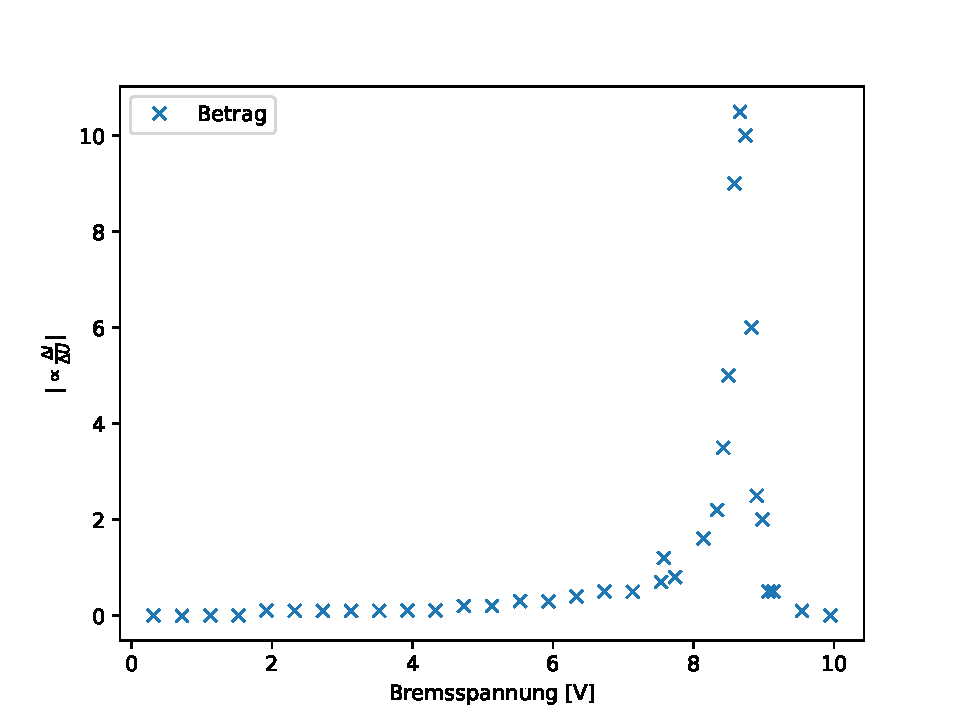
\includegraphics[width = 0.8\textwidth]{Steigung1.pdf}
                  \caption{In der Abbildung ist die differentielle Energieverteilung der ausgelösten Elektronen bei einer Temperatur von 300,85 Kelvin in Abhängigkeit von der Bremsspannung aufgetragen, an der Stelle der größten Steigung lässt sich das Kontaktpotential ablesen.}
                  \label{fig:Steigung300}
                \end{figure}

            \FloatBarrier

            \noindent

            Aus der obrigen Grafik \ref{fig:Steigung300} lässt sich ablesen, dass die Großzahl der Elektronen eine Energie von 8,7 eV besitzt. Da die Beschleunigungsspannung konstant 11 Volt beträgt,
            lässt sich das Kontaktpotential, welches nach der Theorie die Differenz dieser beiden Größen ist, als 2,3 Volt bestimmen.

            \FloatBarrier

                \begin{figure}[h]
                  \centering
                  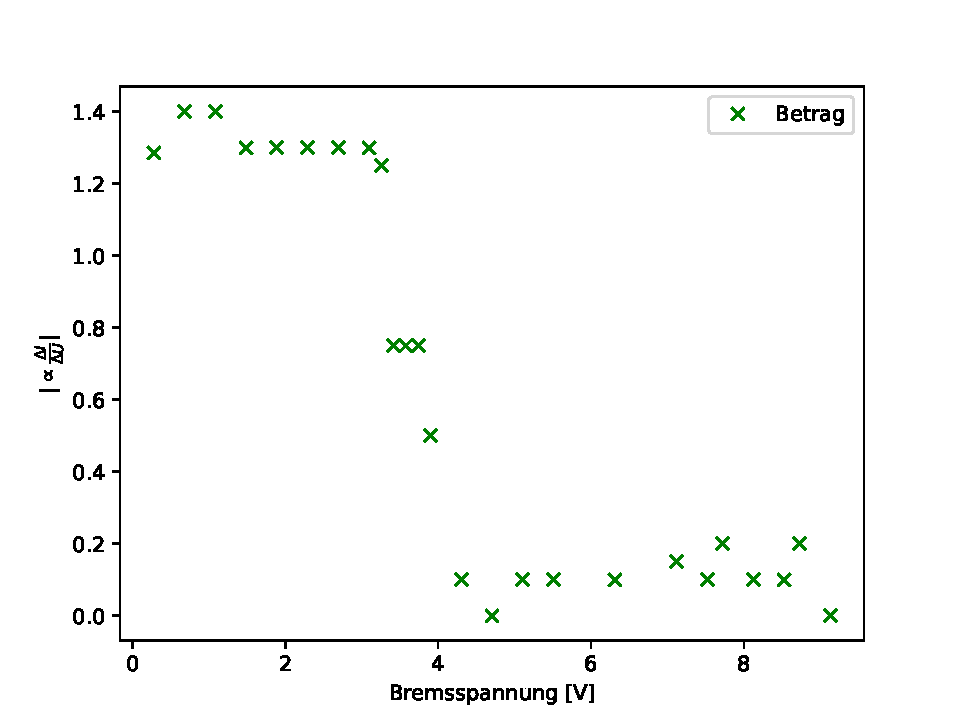
\includegraphics[width = 0.8\textwidth]{Steigung2.pdf}
                  \caption{In der Abbildung ist die differentielle Energieverteilung der ausgelösten Elektronen bei einer Temperatur von 424,15 Kelvin in Abhängigkeit von der Bremsspannung aufgetragen.}
                  \label{fig:Steigung424}
                \end{figure}

            \FloatBarrier

            \noindent

            In der Grafik zur Temperatur von 424,15 Kelvin \ref{fig:Steigung424} lässt sich ein solcher Peak nicht ausfindig machen, da die freie Weglänge nun stark eingeschränkt ist und elastische 
            Stöße die Geschwindigkeit bzw. Energie der Elektronen zufällig verändern. Das plötzliche Absinken geschieht, wenn die Energie der Elektronen genügt, um die Atome anzuregen. 
            Dabei verlieren sie ihre gesamte Energie, sodass nur wenige Atome mit einer höheren Energie gemessen werden können.

        \newpage
        \subsection{Die Franck-Hertz-Kurven}

            \FloatBarrier

                \begin{figure}[h]
                  \centering
                  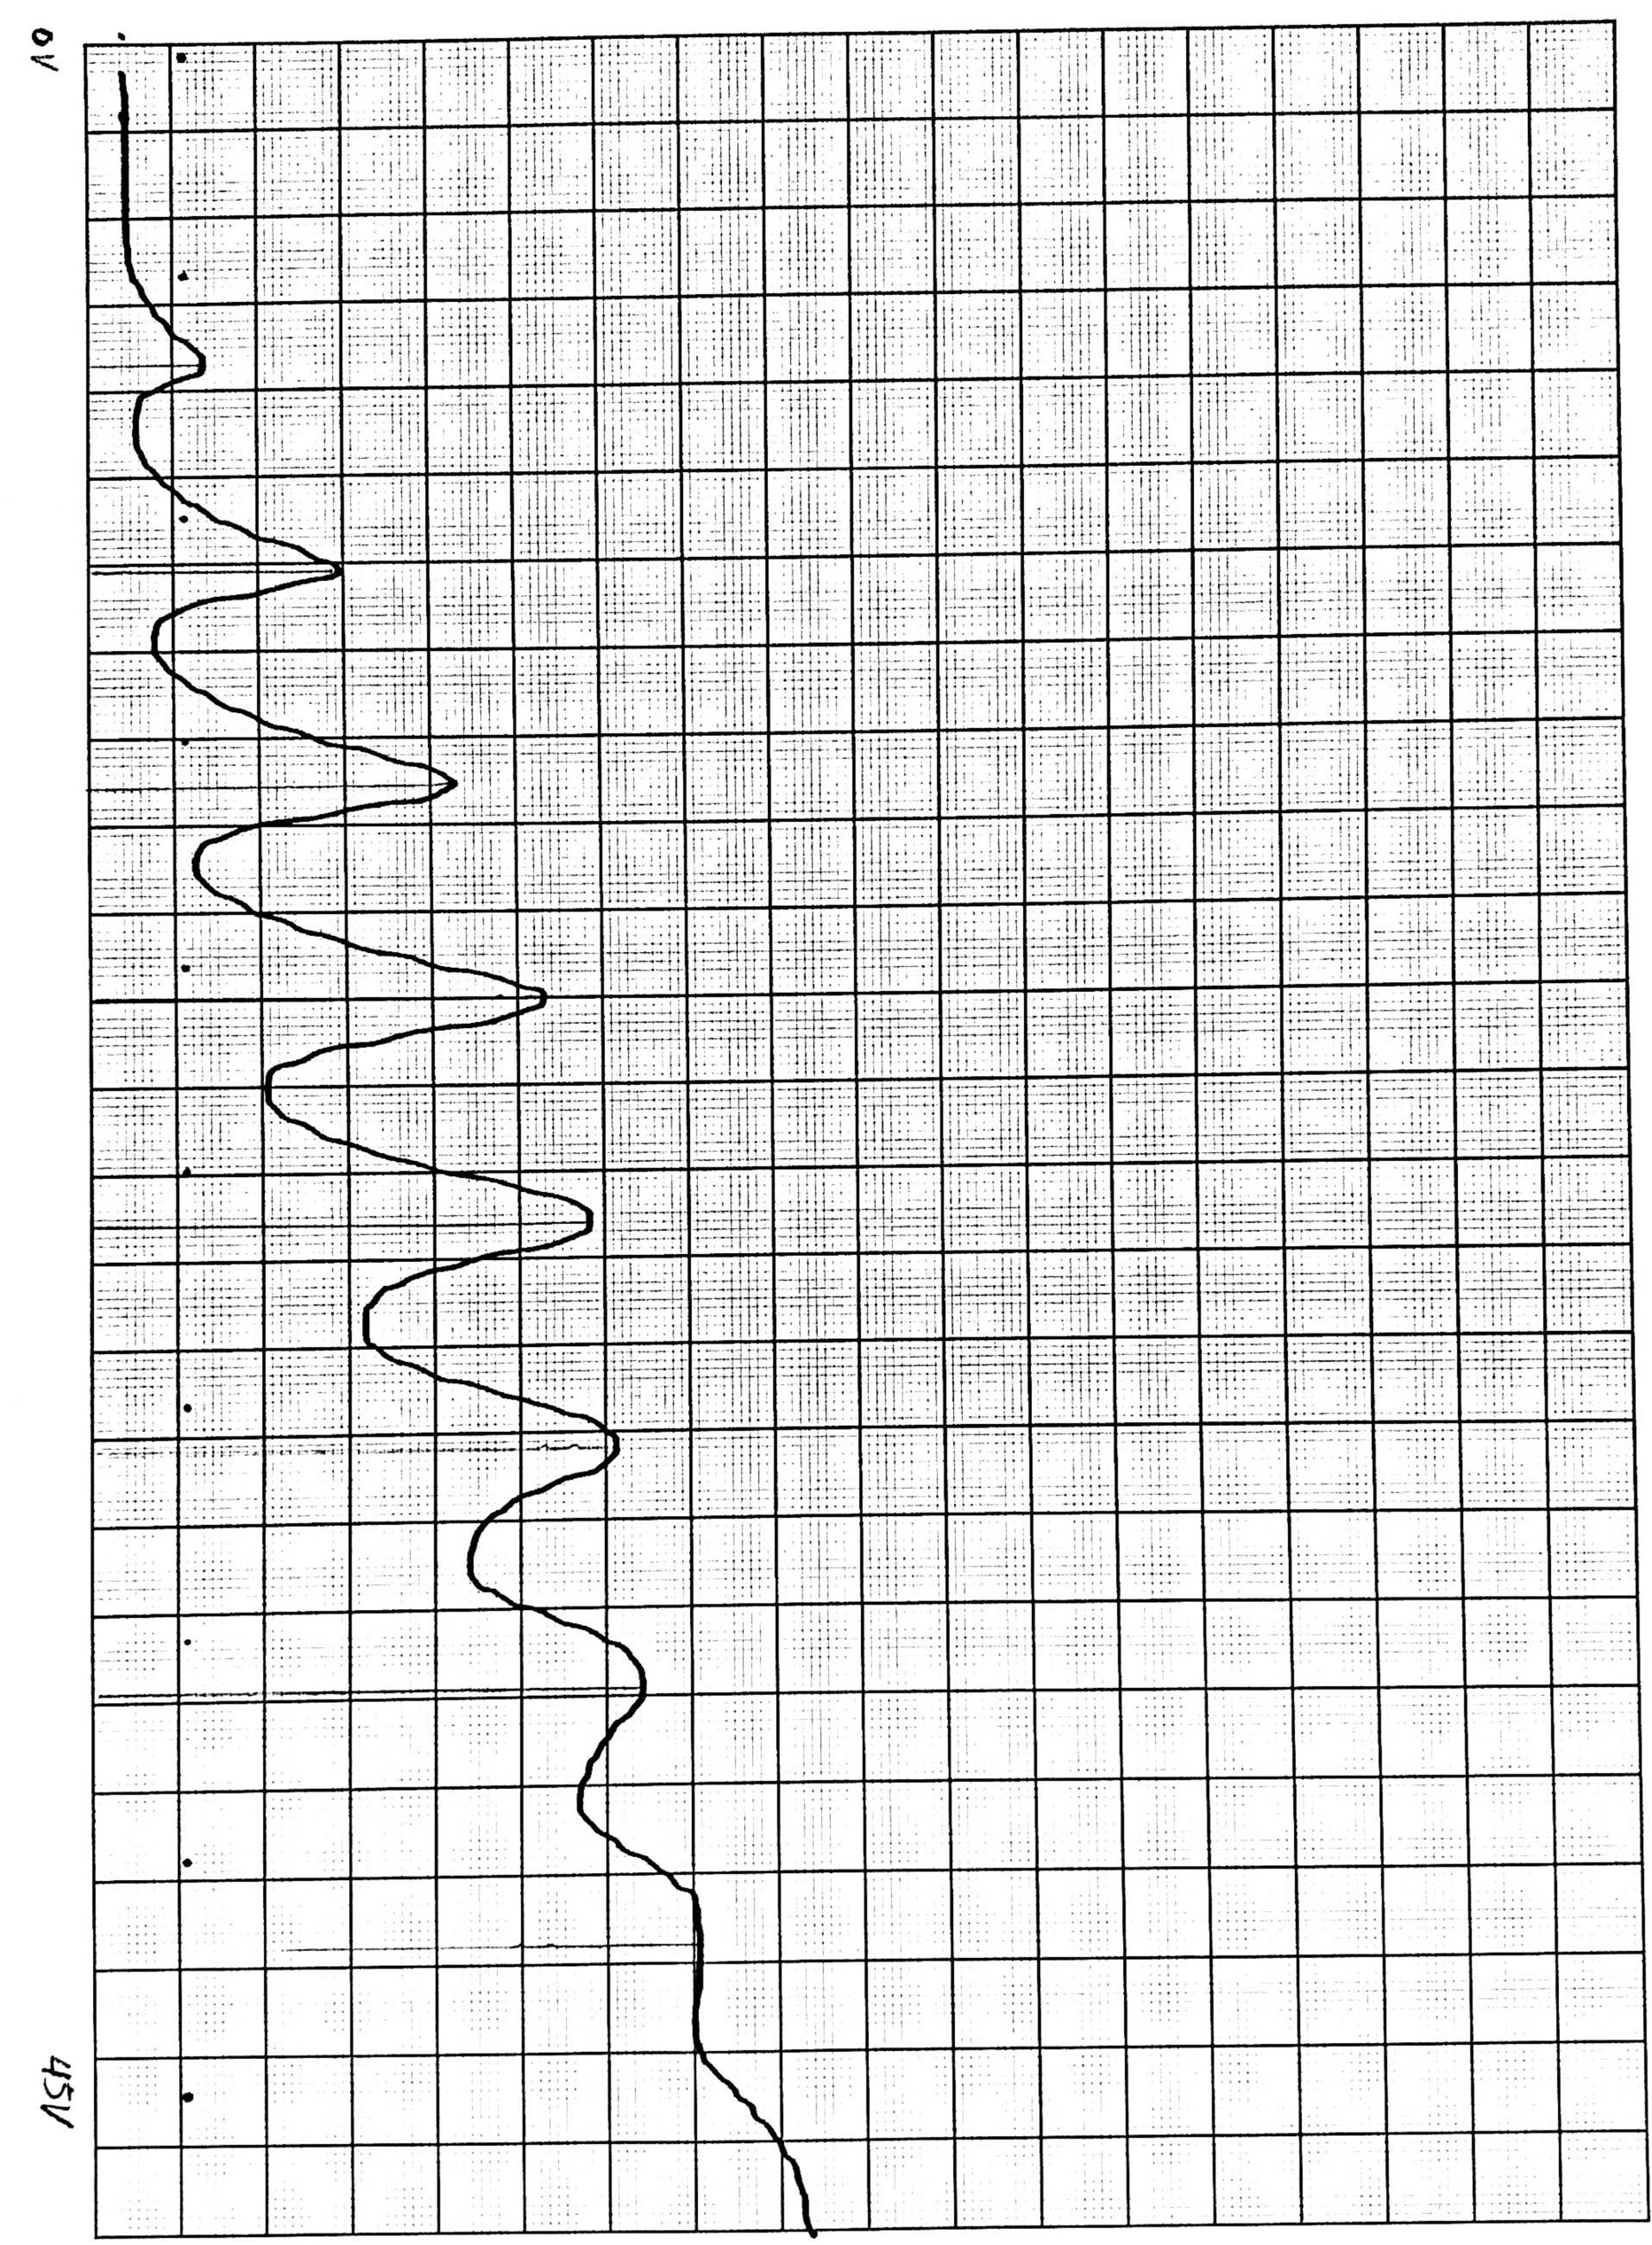
\includegraphics[width = 0.5\textwidth, angle=90]{HertzBild.pdf}
                  \caption{In der Abbildung ist die vom xy-Schreiber aufgenommene Franck-Hertz-Kurve bei einer Temeperatur von 470,25 Kelvin zu sehen.}
                  \label{fig:Steigung300}
                \end{figure}

            \FloatBarrier

            \noindent

            Zunächst wird mit dem selben Vorgehen wie im Abschnitt zur Energieverteilung der losgelösten Elektronen die x-Skala bestimmt. Der einzige Unterschied besteht darin, dass nun die Anzahl an
            Kästchen pro 5 Volt und nur die eine Temeperatur von 470,25 Kelvin betrachtet wird.


            \begin{table}[h]
                \centering
                \caption{In der Tabelle sind zunächst die Anzahlen der Kästchen zwischen den 5V-Markierungen zu sehen. Aus diesen wurde die durchschnittliche Skalierung der x-Achse in mV/Kästchen berechnet.}
                \label{tab:Tabelle1}

                \begin{tabular}{c c}
                    \toprule
                    {} & {470,25 K}  \\
                    \midrule
                    Kästchen/5V   & 24  \\
                                  & 27  \\
                                  & 25  \\
                                  & 25  \\
                                  & 23  \\
                                  & 26  \\
                                  & 26  \\
                                  & 24  \\
                                  & 26  \\
                    \o \; mV/Kästchen & 20,0  \\
                    \bottomrule
                \end{tabular}

            \end{table}

            \FloatBarrier
            \noindent
            Nun lässt sich der Abstand zwischen den Maxima der Kurve in Volt ablesen und somit die erste Ionisationsenergie der Quecksilberatome berechnen. Dazu wird Formel ref nach $\Delta E$ 
            umgestellt und es ergeben sich die folgenden Werte für die Ionisationsenergie. Zudem wird auch die Wellenlänge der Photonen berechnet, die ausgesendet werden, wenn die angeregten 
            Elektronen zurück in den Grundzustand springen.

            \begin{table}[h]
                \centering
                \caption{In der Tabelle ist der Abstand der Beschleunigungsspannung zwischen den Strommaxima, sowie die daraus berechnete Ionisationsenergie des Quecksilberatoms und die zugehörige Photonenwellenlänge beim Zurückspringen des angeregten Elektrons in die ursprüngliche Schale eingetragen.}
                \label{tab:TabelleHertz}

                \begin{tabular}{c c c}
                    \toprule
                    {$\Delta$ U [V]} & {$\Delta$ E [eV]} & {$\Delta \, \lambda$ [$\mu \text{m}$]} \\
                    \midrule
                        4,79 & 4,79 & 25,89 \\
                        4,99 & 4,99 & 24,85 \\
                        4,99 & 4,99 & 24,85 \\
                        5,19 & 5,19 & 23,89 \\
                        5,19 & 5,19 & 23,89 \\
                        5,39 & 5,39 & 23,01 \\
                        5,79 & 5,79 & 21,42 \\
                    \bottomrule
                \end{tabular}

            \end{table}

            \FloatBarrier
            \noindent
            Die durchschnittlichen Werte ergeben sich zu

            \begin{equation*}
                \overline{\Delta \text{U}} = 5,19 \, \text{V} \qquad \overline{\Delta \text{E}} = 5,19 \, \text{eV} \qquad \overline{\Delta \lambda} = 23.97 \, \mu \text{m.}
            \end{equation*}

        
    \newpage
    \section{Diskussion}
        Die Betrachtung der Messergebnisse zeigt eine deutliche Abweichung der Messergebnisse von 50 bis 100 Prozent zu den Literaturwerten. Dies lässt sich nicht direkt erklären. Ein möglicher 
        Störfaktor besteht darin, dass die Messung bei einer Temperatur von 470,25 Kelvin durchgeführt wurde. Dies führt zu einer eigentlich zu geringen mittleren Weglänge. Da die Minima und 
        Maxima dennoch gut zu erkennen sind, wurde die Messreihe bei dieser hohen Temperatur gewählt.






        \FloatBarrier
            
        \begin{table}[h]
          \centering
          \caption{In der Tabelle werden die Messwerte mit den Literaturwerten verglichen.}
        
          \begin{tabular}{c c c c}
              \toprule
              {Messgröße} & {Messwert} & {Literaturwert} & {Abweichung [\%]}\\
              \midrule
        
              $\Delta$U [V]                & 5,19    & 10,44  & 50,29 \%    \\
              $\Delta E_1$ [eV]             & 5,19  & 10,44 & 50,29 \%       \\
              $\Delta \lambda_1 $ [$\mu$m]   & 23,97     & 11,88  & 101.76 \%    \\
              Kontaktpotential [V]         & 2,3  & - &  -                  \\
              \bottomrule
          \end{tabular}
        \end{table}
  
        \FloatBarrier



    \section{Literaturverzeichnis}
        [1] \textit{Versuchsanleitung V601 - Der Franck-Hertz-Versuch.} TU Dortmund, 2020 \newline


    \section{Anhang}

        \begin{table}[h]
            \centering
            \caption{In der Tabelle sind die aus dem Diagramm des xy-Schreibers abgelesenen Werte zur Bestimmung der differentiellen Energieverteilung eingetragen für die Temperaturen 300,85 Kelvin und 424,15 Kelvin.}
            \label{tab:Tabellexy}
           
            \begin{tabular}{c c c c c c}
                \toprule
                {$\Delta I_{300,85}$ [Kästchen]} & {$\Delta U_{300,85}$ [Kästchen]} & {$\frac{\Delta I}{\Delta U}$} & {$\Delta I_{424,15}$ [Kästchen]} & {$\Delta U_{424,15}$ [Kästchen]} & {$\frac{\Delta I}{\Delta U}$}\\
                \midrule
                    0 & 8 & 0 & 9 & 7 & 1,29\\
                    0 & 10 & 0 & 14 & 10 & 1,40\\
                    0 & 10 & 0 & 14 & 10 & 1,40\\
                    0 & 10 & 0 & 13 & 10 & 1,30\\
                    1 & 10 & 0,10 & 13 & 10 & 1,30\\
                    1 & 10 & 0,10 & 13 & 10 & 1,30\\
                    1 & 10 & 0,10 & 13 & 10 & 1,30\\
                    1 & 10 & 0,10 & 13 & 10 & 1,30\\
                    1 & 10 & 0,10 & 5 & 4 & 1,25\\
                    1 & 10 & 0,10 & 3 & 4 & 0,75\\
                    1 & 10 & 0,10 & 3 & 4 & 0,75\\
                    2 & 10 & 0,20 & 3 & 4 & 0,75\\
                    2 & 10 & 0,20 & 2 & 4 & 0,50\\
                    3 & 10 & 0,30 & 1 & 10 & 0,10\\
                    3 & 10 & 0,30 & 0 & 10 & 0\\
                    4 & 10 & 0,40 & 1 & 10 & 0,10\\
                    5 & 10 & 0,50 & 1 & 10 & 0,10\\
                    5 & 10 & 0,50 & 2 & 20 & 0,10\\
                    7 & 10 & 0,70 & 3 & 20 & 0,15\\
                    4 & 5 & 0,80 & 1 & 10 & 0,10\\
                    6 & 5 & 1,20 & 1 & 5 & 0,20\\
                    8 & 5 & 1,60 & 1 & 10 & 0,10\\
                    11 & 5 & 2,20 & 1 & 10 & 0,10\\
                    7 & 2 & 3,50 & 1 & 5 & 0,20\\
                    10 & 2 & 5,00 & 0 & 10 & 0\\
                    18 & 2 & 9,00 & & &\\
                    21 & 2 & 10,50 & & &\\
                    20 & 2 & 10,00 & & &\\
                    12 & 2 & 6,00 & & &\\
                    5 & 2 & 2,50 & & &\\
                    4 & 2 & 2,00 & & &\\
                    1 & 2 & 0,50 & & &\\
                    1 & 2 & 0,50 & & &\\
                    1 & 10 & 0,10 & & &\\
                    0 & 10 & 0 & & &\\

                \bottomrule
            \end{tabular}
           
        \end{table}
       
        \FloatBarrier
        \noindent


            
            
            
            


        \end{document}